% !TEX TS-program = pdflatex
% !TEX encoding = UTF-8 Unicode

% This is a simple template for a LaTeX document using the "article" class.
% See "book", "report", "letter" for other types of document.

\documentclass[11pt]{report} % use larger type; default would be 10pt

\usepackage[utf8]{inputenc} % set input encoding (not needed with XeLaTeX)
\usepackage{listings}

%%% Examples of Article customizations
% These packages are optional, depending whether you want the features they provide.
% See the LaTeX Companion or other references for full information.

%%% PAGE DIMENSIONS
\usepackage{geometry} % to change the page dimensions
\geometry{a4paper} % or letterpaper (US) or a5paper or....
% \geometry{margin=2in} % for example, change the margins to 2 inches all round
% \geometry{landscape} % set up the page for landscape
%   read geometry.pdf for detailed page layout information

\usepackage{graphicx} % support the \includegraphics command and options

\usepackage[parfill]{parskip} % Activate to begin paragraphs with an empty line rather than an indent

%%% PACKAGES
\usepackage{booktabs} % for much better looking tables
\usepackage{array} % for better arrays (eg matrices) in maths
\usepackage{paralist} % very flexible & customisable lists (eg. enumerate/itemize, etc.)
\usepackage{verbatim} % adds environment for commenting out blocks of text & for better verbatim
\usepackage{subfig} % make it possible to include more than one captioned figure/table in a single float
\usepackage{float}
\usepackage[toc]{appendix}
\usepackage{multirow}
\usepackage[backend=bibtex]{biblatex}
\usepackage[export]{adjustbox}
% These packages are all incorporated in the memoir class to one degree or another...

%%% HEADERS & FOOTERS
\usepackage{fancyhdr} % This should be set AFTER setting up the page geometry
\pagestyle{fancy} % options: empty , plain , fancy
\renewcommand{\headrulewidth}{0pt} % customise the layout...
\lhead{}\chead{}\rhead{}
\lfoot{}\cfoot{\thepage}\rfoot{}

%%% SECTION TITLE APPEARANCE
\usepackage{sectsty}
\allsectionsfont{\sffamily\mdseries\upshape} % (See the fntguide.pdf for font help)

\usepackage{titlesec}
\titleformat{\chapter}[display]{\normalfont\bfseries}{}{0pt}{\Large}
%\titlespacing*{\chapter}{0pt}{1.1\baselineskip}{\baselineskip}

%\makeatletter
%\renewcommand\chapter{\thispagestyle{plain}%
%	\global\@topnum\z@
%	\@afterindentfalse
%	\secdef\@chapter\@schapter}
%\makeatother

% (This matches ConTeXt defaults)

%%% ToC (table of contents) APPEARANCE
\usepackage[nottoc,notlof,notlot]{tocbibind} % Put the bibliography in the ToC
\usepackage[titles,subfigure]{tocloft} % Alter the style of the Table of Contents
\renewcommand{\cftsecfont}{\rmfamily\mdseries\upshape}
\renewcommand{\cftsecpagefont}{\rmfamily\mdseries\upshape} % No bold!

%%% END Article customizations

\addbibresource{bibliography.bib}

%%% The "real" document content comes below...

\begin{document}

\begin{titlepage}
	\begin{center}
	\large
	University of Manchester\\
	School of Computer Science\\
	\vspace{1.5cm}
	\vspace*{1cm}
	\Large
	NetProtect:\\
	Malware Detection and Remote Quarantine Solution\\
	for an Enterprise Environment\\
	\normalsize
	Third Year Project
	
	\vspace{1.5cm}
	
	\large
	Author: Corey Arthur, Bsc. Computer Science\\
	Supervisor: Dr Ning Zhang, PhD
	
	\vfill
	April, 2018
	
\end{center}
\end{titlepage}


\newpage

\begin{abstract}
	Since the early invention of desktop computers, computer viruses have been developed and deployed around the globe. What may have started as a proof of concept exploration into the ability for computer programs to self-replicate is currently thought to cost billions of dollars’ worth of damage each year. In 2017 alone, Panda Security reported more than 15 million different malicious portable executable files had been identified with a 50\% increase in ransomware appearances from 2016. Of these malicious portable executables 99.10\% were identified as unique \cite{panda}. With the increasing trend of network propagation as a means to spread malware, the need for a combined antivirus and remote quarantine facility in a business environment is ever increasing.
	
	This project covers the development of NetProtect, a next generation malware detection and remote quarantine suite. Focusing on preventing infected systems from spreading to the remaining infrastructure whilst providing a modular interface to enable augmentation with new detection techniques, future-proofing the facility against the ever changing malware development ecosystem.
	
	<<TODO BETTER FINDINGS/LESSONS PARAGRAPH>>
	
	This report will discuss the growing issue of malicious software and demonstrate the need for a new era of antivirus solutions incorporating dynamic network quarantining to help prevent the spread of network-propagating malware. Additionally, the report aims to highlight the advantages of a modular antivirus solution to enable malware detection to maintain pace with the ever-changing malware development ecosystem.
\end{abstract}

\renewcommand{\abstractname}{Acknowledgements}
\begin{abstract}
	...
\end{abstract}

\tableofcontents

\chapter{Introduction}
	While the first developed viruses may have only been designed as practical jokes to confuse, the incorporation of computer systems into business procedures and the popularization of the public internet provided the perfect opportunity for malware development to shift towards a more malicious payload. These payloads are designed to steal and/or destroy data held by the businesses but have been built upon over decades with new infection and spreading techniques and varied objectives. This may be as simple as creating a remote storage server to host stolen data to initiating compromised servers into a botnet, which may be used to disable remote network infrastructure through synchronized carried out by hundreds of compromised devices.	
	
	Since the first malicious program was released, threat actors have reverse-engineered protocols, popular software and operating systems in hopes of finding a zero-day exploit. Such an exploit is one which has not yet been discovered and subsequently patched. These exploits would therefore allow attackers to infect many more machines than relying on targets with systems not containing the latest security patches. In the case of exploits targeting network protocols this creates a significant opportunity for threats to spread from a single infected computer to the rest of the network connected devices which utilise the protocol.
	
	With the recent leak of the NSA’s ETERNALBLUE zero-day exploit, targeted at the SMB protocol implementation available on Microsoft Windows devices and similar emerging network protocol exploits the need for an anti-virus solution which has the ability to remotely quarantine an infected device from a network is ever increasing.
	
	Traditionally, antivirus solutions have focused on detecting viruses on a single machine through the use of basic detection techniques which may be carried out on the protected system without need for an analysis server. However, as malware complexity increases it is becoming less feasible for the analysis routines to take place on the system. Therefore, it is becoming more common for clients to perform basic analysis on their system before sending the results to a central server for more detailed analysis. In business environments where data stored may comprise of sensitive data, this approach cannot be used as it can never be ensured that the data sent for analysis does not compromise the sensitive data. It is for this reason that the availability of an antivirus solution which can be deployed by a business would be invaluable.
	
	It is from these issues such that this project aims to investigate the feasibility of a self-hosted antivirus solution which can be expanded upon with the latest detection techniques. <ADD MORE HERE>
	
	\section{Malware Detection Techniques: an Overview}
		In the early days of malware, the number of known malware samples was relatively small. Though due to the large attack surface available its use in cyber crime has spurred its development, rapidly increasing the number of samples year after year. As a result, new methods are constantly being developed to be able to classify previously unseen families of malware using advanced techniques employing artificial intelligence.
		
		\subsection{Hash Based}
			As the number of malicious programs began to rise, it was clear that a solution was needed which would allow files to be classified. The simplest of these was to utilise a hashing algorithm to produce an identifier for a file’s contents. As new samples were discovered, their identifiers (file hashes) were added to a database which could then be queried to determine a files classification. However, this required the file to have been previously encountered and was fully reliant on the files contents being identical. As a result, developers began to create many different variants of their malware, each containing a different token and therefore resulting in a different hash.
		\subsection{Byte Signature Based}\label{intro.bytesignaturetechnique}
			Designed partially to combat the issues of hash-based techniques, byte signature instead stores common signatures which have been found to be present in malicious programs. These may be identifiers such as segments of a ransomware letter or anonymous bitcoin addresses for ransom payments to be sent to. Some tools allow multiple byte signatures to be combined with Boolean logic to create more robust rule sets to increase their accuracy.
		\subsection{Heuristics Based}
			By extracting features from files such as their metadata or the sections contained in the executable (.text, .code, etc) machine 	learning can be used to analyse the extracted features against those found within known malicious files to classify previously unseen samples. One heuristic which was often used by earlier antivirus systems was the “Entry Point” set by the executable which determined the offset at which the operating system began execution of the file. This was effective as malware which spreads to other files often appends the malicious code to the end of the legitimate executable and changes the entry point to that of the new malicious code. Alternatively, packers which encrypt malware to prevent static analysis and only decrypt the executable contents tend to have large .text sections consisting of encrypted code and short .code sections which comprise of the decryption routines.
		\subsection{Behavioural Analysis Based}
			In cases where obfuscation tools have been used to try to hide the inner workings of a program, or where programs have been ‘packed’ to encrypt the payload, behavioural analysis techniques can be used to inspect files and binaries in a dynamic environment. First of all, the file is sandboxed to allowing the program to run without modifying any files on the system. While in this sandbox, the program is allowed to operate as designed while the host system captures all interaction between the host and the malware. This information can then be analysed, possibly in combination with heuristics obtained through static analysis to classify the binary.


\chapter{NetProtect Design}

	With traditional antivirus products focusing on the protection of individual devices, their use in a business context as a front-line solution lacks the benefits of a central management interface. This leaves the security of the systems down to the user, who may forget, or not care to routinely perform antivirus scans.
	
	NetProtect is instead designed to allow clients to be managed remotely, taking the responsibility from the user and providing a platform for which client scans can be analysed off-device with the future possibility of remotely initiating scans on a routine basis, or automatically quarantining systems which have not been scanned for an extended period of time.
	
	\section{Architecture Overview}
		As NetProtect has the functionality to make major changes to the network environment, the design architecture had to be considered from a security perspective. Therefore its architecture has been designed as a thin-client for use on host machines, reducing the attack surface available should a malicious actor gain access to a system, with a central server used to analyse the files submitted by the client.
		
		Since it was decided that a functional requirement of the system was the ability to interface with a gateway or firewall to allow remote quarantining of an infected device from the network, the use of a client-server architecture would be the most suitable approach as this would mean only the server would have the credentials required to issue the instruction to quarantine a client from the network.
		
		Alongside the security considerations, the use of a client-server architecture would open further avenues to explore such as the ability to monitor scan occurrences to identify clients which were not routinely scanning their system, and the ability to deploy schedules for clients to follow. Though these were not implemented but are discussed later in the report in section \ref{FutureImprovements.AnalysisServer}. 
		
		Figure \ref{fig:systemarchitecture} shows how each component is connected, from which it can be seen how the client is treated as an untrusted entity preventing rogue access to the database and firewall components.
		
		
		\begin{figure}[H]
			\begin{center}
				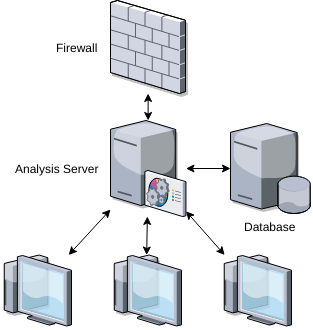
\includegraphics[scale=0.5]{images/systemarchitecture.png}
				\caption{NetProtect solution architecture.}
				\label{fig:systemarchitecture}
			\end{center}
		\end{figure}
	
		\subsection{Scanning Procedure}
			When a user initiates a scan and selects the folders to be scanned, the client system creates a new scan task using the scan module selected by the client. This allows a range of scans to be performed by the client should they wish to execute a specific scan. For example, a user may simply wish to perform a hash scan on a large file or a multi-technique scan on the entire computer.
			
			\subsubsection{Scan Process}
			Once the task has been created, the scan manager sends it to the task scheduler to be executed once a thread becomes available. The system will then traverse the chosen directories creating a new subtask for each file and queueing them into the task scheduler.
			
			As a file is processed by the system, the features extracted are stored in a report which is sent to the server at a suitable interval. By default, this is set to occur once the scan report contains around one hundred items. This aims to minimise the time wasted initiating the session without the server having to hold a socket open for a client when others may potentially be ready to submit, without delaying the scan process by waiting for all files to be processed before submission.
			
			\subsubsection{Report Submission}
			To submit a scan report, the scan manager creates a network task to begin communication with the server. This task performs the necessary session initiation with the server and sends an analysis command along with the scan report encoded in a JSON representation. Once the submission is confirmed by the server the connection is closed, the scan manager will record the identifier of the report and periodically query the analysis server for the results.
			
			\subsubsection{Analysis}
			When an analysis request is received by the server, an analysis task is created for the appropriate module and sent to the task scheduler. The implementation of the analysis task will then consider the features extracted for a file to determine how it should be classified. As with the scan module, this process may use external tools such as the submission to a cloud analysis platform or other techniques. In the case a malicious file is detected, the analysis manager will be notified by the task which may then request the quarantine of the device from the network.
	
	\section{Architecture in Detail}
		\subsection{Client Architecture}
			As the client is designed to simply extract the features required by the server for analysis, its architecture is simple. Figure \ref{fig:clientarchitecture} displays the structure of the underlying components, with its functionality revolving around the Scan Manager component. As clients initiate a scan via the interface, the Scan Manager generates the scan task from the chosen Scan Module and queues it for execution by the Task Scheduler. As the task begins generating reports to be analysed by the server, the Scan Manager stores the report reference before the Connection Manager sends the report for analysis. 
			
			Once reports have been sent for analysis, it is the job of the Scan Manager to periodically retrieve the results from the server.
			
			\begin{figure}[H]
				\begin{center}
					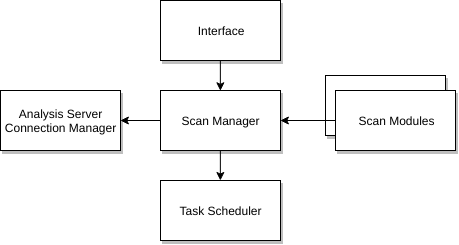
\includegraphics[scale=0.7]{images/clientarchitecture.png}
					\caption{NetProtect client architecture.}
					\label{fig:clientarchitecture}
				\end{center}
			\end{figure}
		
			\subsubsection{Interface}
				To enable the user to interact with the system in an efficient manner, a simple user interface was required providing the functions of initiating a scan, and informing the user of the state of existing in-progress scans. 
				
				Figure \ref{fig:clientinterface} displays the general user interface showing some system statistics, and the general status of the current task. 
				
				A more detailed view of the scan tasks can be seen in figure \ref{fig:clientscaninterface} displaying the files being scanned, their status and where files have already been scanned, their classification. Additionally, a panel containing information on the report submission process is displayed below.
				
				\begin{figure}[H]
					\begin{center}
						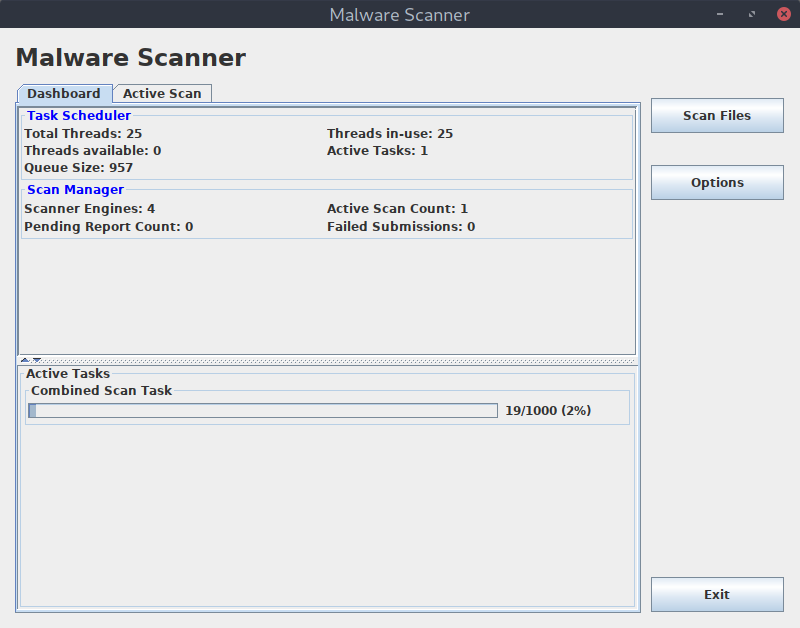
\includegraphics[width=\linewidth,frame]{images/clientinterface.png}
						\caption{NetProtect client interface.}
						\label{fig:clientinterface}
					\end{center}
				\end{figure}
				
				\begin{figure}[H]
					\begin{center}
						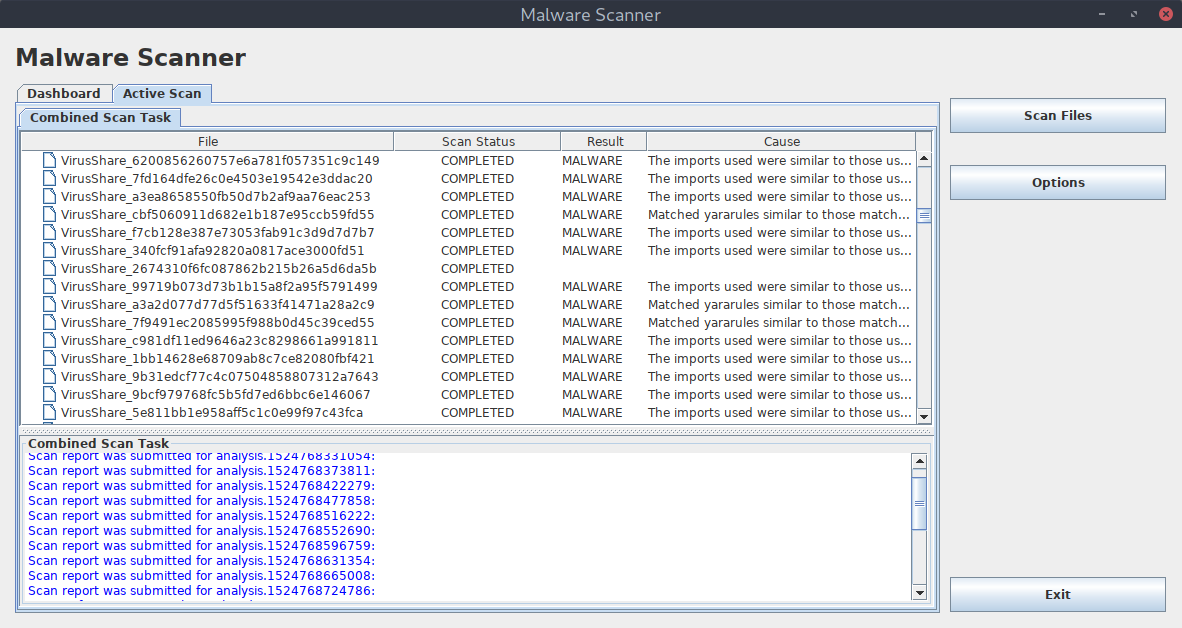
\includegraphics[width=\linewidth,frame]{images/clientscaninterface.png}
						\caption{NetProtect client scan interface.}
						\label{fig:clientscaninterface}
					\end{center}
				\end{figure}
			
			\subsubsection{Scan Modules}
				As malicious actors constantly discover new techniques to spread and utilise malware, it is necessary that those defending against such threats also innovate upon detection techniques. As a result, in recent years anti-virus solutions have shifted towards new signature-less detection techniques, however these techniques are still constantly evolving. 
				
				While NetProtect will not be in long term or production use, it was decided that for the solution implemented to qualify as successful it must be easily extensible to allow custom file scanning and analysis techniques to be created and integrated into the system. Doing so would enable the solution to keep pace with the ever-changing malware ecosystem, futureproofing its ability to detect and classify malware.
			
			\subsubsection{Hash Based Scan Module}
				The most simple of the scan modules, the hash based scan determines the file classification by calculating the file hash, and submitting it to the server. 
			\subsubsection{Byte Signature Based Scan Module}\label{client:bytesignature}
				As with the technique described in section \ref{intro.bytesignaturetechnique}, comparing the file content to byte signatures provided by malware researchers allows simple observations to be made about a files operation. This module extracts 'interesting' byte signatures, which are sent to the server for analysis. 
			\subsubsection{Import Heuristic Based Scan Module}\label{client:importheuristic}
				An experimental scan technique, the import heuristics scan module extracts the functions imported from a portable executable file to attempt to determine the executables purpose. The list of features extracted from portable executable files are sent to the server for classification. However if the file is not a portable executable file, or does not have an import section it will be skipped. 
			\subsubsection{Combined Technique Scan Module}
				While the hash based detection technique is quickly becoming ineffective, its effectiveness at detecting known malware is unrivalled, therefore the combined technique uses each of the implemented modules in order, ensuring all known malware is detected, with a fallback to newer heuristic techniques.
			
		\subsection{Server Architecture}
			
			\begin{figure}[H]
				\begin{center}
					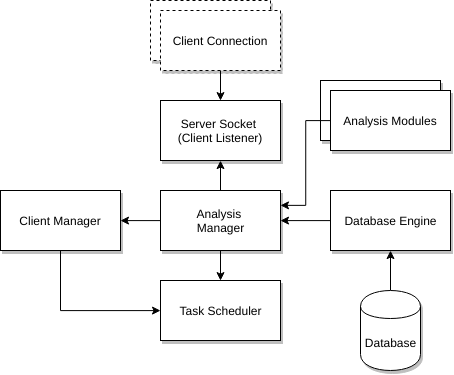
\includegraphics[scale=0.7]{images/serverarchitecture.png}
					\caption{NetProtect server architecture.}
					\label{fig:serverarchitecture}
				\end{center}
			\end{figure}
			
			As seen in figure \ref{fig:serverarchitecture}, the server architecture is built around the central component, the analysis manager. Firstly, clients connect with the Server Socket component which processes the requests made and transmits them to the analysis manager. These requests are then recorded by the analysis manager and queued for execution within the task scheduler. 
			
			In the case malware is detected during analysis, the analysis manager will then notify the client manager, which will in turn generate a task to quarantine the client, which will then be queued for execution with the highest priority.
			
			\subsubsection{Interface}
				While the server architecture is primarily designed as an automated component, as this is the core component of the system the decision was made to provide system administrators with a simple interface to view the status of ongoing tasks, a statistics panel to give a quick overview of the usage, and a simple control interface to remove clients from quarantine once the threat has been controlled.
				
				\begin{figure}[H]
					\begin{center}
						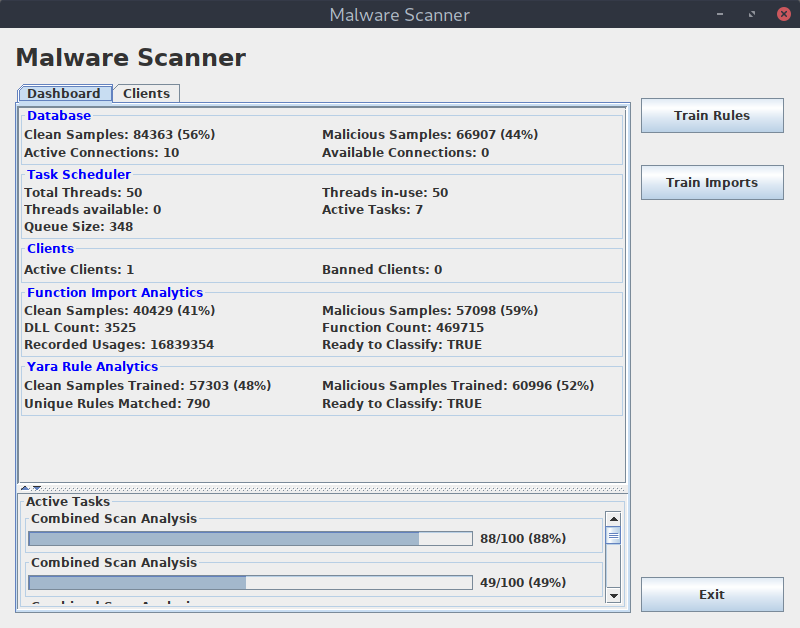
\includegraphics[width=\textwidth,frame]{images/serverinterface.png}
						\caption{NetProtect server interface.}
						\label{fig:serverinterface}
					\end{center}
				\end{figure}
				
				Figure \ref{fig:serverinterface} shows the server interface, with detailed statistics about the systems usage and analysis module state. A number of analysis tasks can be seen processing within the interface.
				
			\subsubsection{C4.5 Algorithm}\label{c45}
				Incorporating machine learning aspects into analysis modules is a key factor in being able to distinguish malicious files in samples which have not previously been encountered and analysed by malware researchers. This allows a classification to be derived from a set of features extracted from a file by comparing with a dataset of features extracted from known malicious and known non-malicious files. The requirements for the algorithm to be used in the project were simple, to support both continuous and discrete features, and to output a binary label to classify the result. The C4.5 algorithm was suitable for this purpose and creates a decision tree which can be easily traversed.
				
				The algorithm implementation is simple, for each feature in the dataset, the entropy is calculated at the current level where the data be split using that feature. The best feature is then selected as the one which provides the highest entropy gain, and recorded as a node in the tree. To optimise the process, three base cases exist to generate a terminal node: all data elements have the same label, the number of data elements is below a threshold, or there exists no data elements in that portion of the tree.
			
			\subsubsection{Hash Based Analysis Module}
				As with the associated scan module, the hash based analysis module is simple. Each file hash submitted by clients is checked for existence in a database of known malicious files, files are classified as malicious only if the signature is present.
			\subsubsection{Byte Signature Based Analysis Module}
				Using the byte signatures matched by the clients during the scanning process, the server utilises the C4.5 algorithm described in section \ref{c45} to classify files using the decision tree generated during the algorithms training phase. The tree is navigated using the extracted matching byte signatures until a terminal node is reached, classifying the file.
			\subsubsection{Import Heuristic Based Analysis Module}
				As with the byte signature based analysis module, the algorithm uses the C4.5 algorithm to classify files. The decision tree is navigated with the path taken chosen as a result of the imported functions within the portable executable file. The terminal node at which the tree arrives is the resulting classification of the file.
			\subsubsection{Combined Technique Analysis Module}
				To overcome the shortfalls of the other techniques, the combined analysis module performs hash based, byte signature based, and import heuristic based analysis in order. Should any of the stages identify the sample as malware, the analysis is completed ignoring the result of the subsequent stages.
		
		\subsection{Firewall Architecture}
		
			\begin{figure}[]
				\begin{center}
					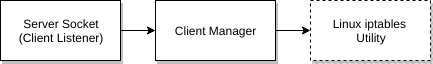
\includegraphics[scale=0.6]{images/firewallarchitecture.png}
					\caption{NetProtect firewall architecture.}
					\label{fig:firewallarchitecture}
				\end{center}
			\end{figure}
		
			The architecture of the firewall element of the NetProtect system displayed in figure \ref{fig:firewallarchitecture} shows the simple composition of the two components required. Firstly, the server socket allows clients to send commands which are processed to instruct the client manager quarantine, or remove clients from the quarantine by interacting with the iptables utility.
			
			\subsubsection{Quarantine Component}
			Originally, the planned implementation of the network quarantine functionality focused on the use of an open source fork of the popular gateway utility PFSense, which advertised the ability to interact with the system through the use of a high-level REST API. However, when looking further into the documentation, it was evident that the API advertised was not as extensive as required. The firewall functionality did not have any available API endpoints and therefore could not be configured remotely. Following this discovery, a number of alternative solutions were investigated.
			
			Firstly, the use of a DHCP server allows clients configured with a dynamic IP address to request an available IP address from the server. By developing a basic DHCP server, a table of clients could be stored along with their associated IP and MAC addresses. To quarantine a system, a DCHPRELEASE instruction would be sent to the host who would then discard the current IP address and request a new address from the server but would be denied. Though this approach relies on all clients being configured with dynamic IP addresses and that they obey DHCPRELEASE instructions.
			
			Alternatively, a DNS client converts domain names requested into the associated IP addresses and are often used within businesses to cache DNS entries to lower the overall number of queries required. A custom DNS client could be configured to respond to queries from quarantined clients with an alternative address, for example a webserver hosted by the company with information as to why the client had been quarantined. However, on a local network malware usually spreads without the use of DNS queries so this approach would not succeed in our requirement of quarantining infected systems.
			
			However, the chosen method was the use of the iptables utility in Linux, a custom client operating at the network gateway was developed to dynamically add and remove rules instructing the system to drop packets originating from or heading towards a quarantined client. This method was deemed the most suitable due to its simplicity, and flexibility. Additionally, connectivity to specific clients such as the antivirus server could be maintained on a “whitelist” basis. Though one issue with this approach requires the assumption that all traffic on the network must travel through the system operating as the firewall regardless of if the clients are currently on the same subnet. 
		

\chapter{NetProtect Implementation}
	With the functionality and architecture requirements decided during the design phase, the final implementation was achieved through a development process which took place over a number of iterations. As the solution also aims to maximise speed, the implementation utilises multithreading techniques allowing the concurrent execution of tasks. This is most evident during the scanning process, as each thread can operate on a separate file in parallel. This is possible due to the use of an Executor which operates as a task scheduler, storing the tasks which are waiting to be executed and distributing them to threads as they are available.
	
	\section{Design Patterns}
	
		\subsection{Template Method Pattern}
			With the aim of code modularity, the implementation uses a ‘Task’ class from which all tasks are derived. To achieve this, the template method pattern was used along with Java inheritance allowing tasks to be created for various purposes, with only implementation specific procedures needing to be written.
			
			\begin{figure}[h]
			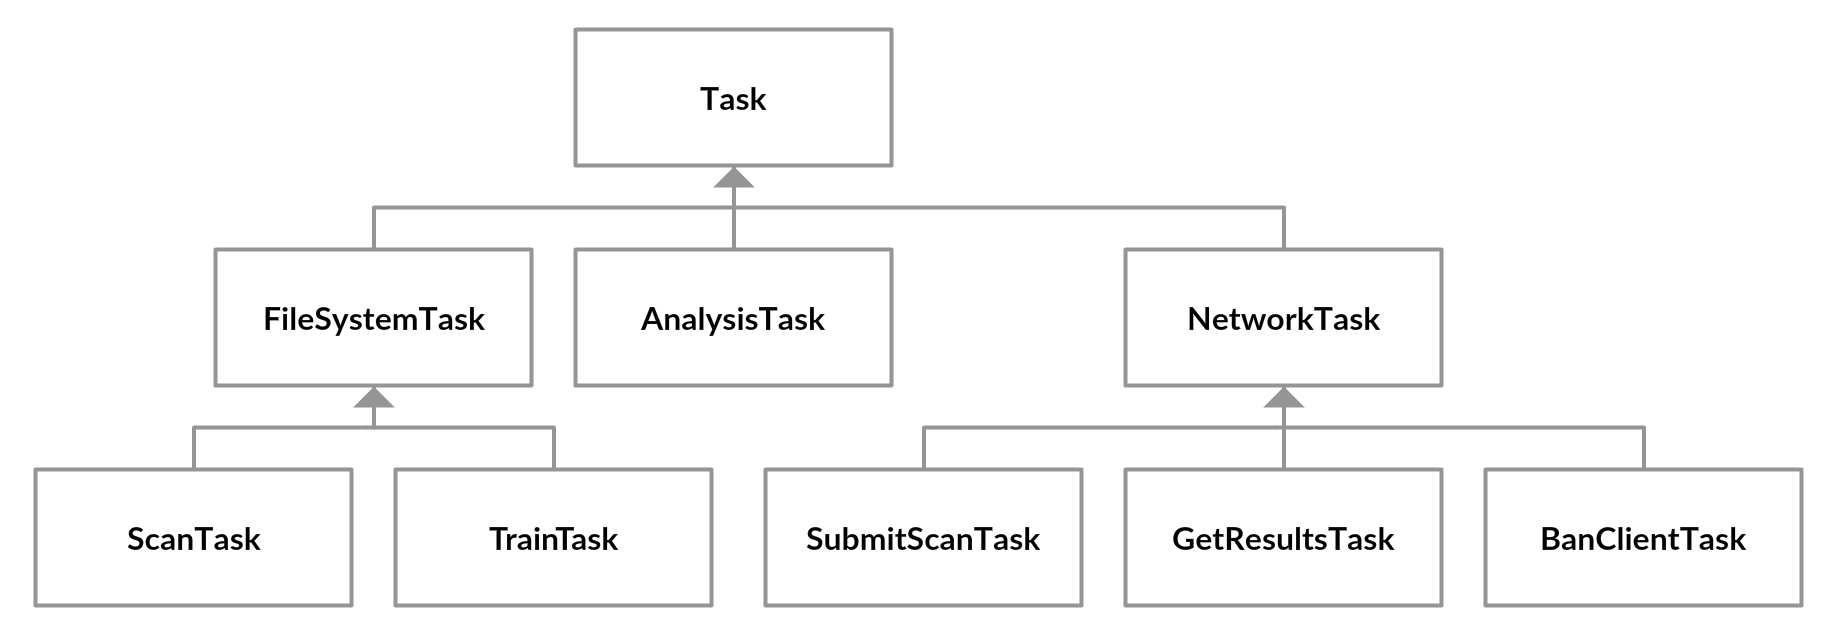
\includegraphics[width=\linewidth]{images/taskhierarchy.png}
			\caption{A subset of the Task class hierarchy.}
			\label{fig:taskhierarchy}
			\end{figure}
			
			Figure \ref{fig:taskhierarchy} shows the task class hierarchy with a small subset of the classes used in the implementation. For example, ScanTask implements FileSystemTask to provide the file system abstraction, allowing its implementation to be as simple as shown in the figure below.
			
			\subsubsection{Scan Task}
				The below code is the minimum template for a scan module which takes a single file and should then extract the features required for classification at the analysis stage. One implementation example may extract the metadata of the file or alternatively, run an external tool such as 7zip to extract compressed files and analyse their contents.
			
				\begin{minipage}{\linewidth}
					\lstinputlisting[frame=single,language=java, caption=Template used to implement a new scan technique]{minscantask.java}
				\end{minipage}
			
			\subsubsection{Analysis Task}
				Similar to the Scan Task, this code is the minimum template for an analysis module. The analysis module uses the features extracted by the corresponding scan module to determine a single files classification. This may be as simple as checking the files hash against a database of malicious files, or a complex analysis using artificial intelligence. Once the classification is complete, the result is added to the results report to be sent back to the client.
			
				\begin{minipage}{\linewidth}
					\lstinputlisting[frame=single,language=java, caption=Template used to define analysis of file features.]{minanalysistask.java}
				\end{minipage}
			
			
			\subsubsection{Network Task}
				As the primary method of communication between client and server or server and firewall, the network task aims to simplify such communication by abstracting the creation of the communication socket, handshake procedure, encryption and decryption routines. For a developer to create such a task, it is necessary only to define which messages to be sent to the server and the result of the task should an exception arise.
				
				Since the software was designed with security considerations in mind, all communication between clients is encrypted. Firstly, clients must be configured with the analysis server’s public key, this is used in the initial handshake procedure as clients generate an ephemeral symmetric key which is encrypted with the public key of the server. The use of a symmetric key allows large messages such as scan reports to be encrypted and decrypted much faster than the use of a public/private key pair. Once received, the server decrypts the key and responds with an encrypted nonce to which the client must decrypt and respond with the nonce-1 to prove the knowledge of the correct key. While this does little from a security perspective in this situation, it enables early detection of a communication error due to the invalid communication of the symmetric key.
	
		\subsection{Observer Pattern}
			To integrate the interface of the client and server components with the state of the various 'tasks' used within NetProtect, the observer pattern was implemented, allowing interface components to subscribe to state updates from other components. For example, the 'Task Scheduler' component notifies listeners of task creation and completion and is used by the active tasks panel to dynamically create and destroy progress panels for the various tasks.
	
	\section{Training Data Acquisition}
		In order to properly train the system in the detection of malware using the various methods planned, a sufficient number of samples of both clean and malicious files were required. As the detection methods implemented required real life samples to properly demonstrate the technique it was infeasible to automate the creation of malicious files with the degree of variation in operation as would be seen in the wild.
		
		Instead the samples were acquired through VirusShare \cite{virusshare}, an online malware repository aimed at malware researchers and security professionals. The site hosts compressed archives each containing thousands of samples of varying types. A number of these were downloaded resulting in 262144 samples, though some scan modules only perform on specific filetypes and to train the modules on all samples would have taken more time than available. As the files were named with only their md5 sum without a filetype, a short script was written utilising the linux file command to identify the file and sort accordingly. Table \ref{tbl:samplecount} shows the types of malware identified after sorting.
		
		Originally, a clean installation of windows 10 was used to train the system however, as with malicious samples, a large quantity of clean samples were required for proper training of the system. Without these, the system would likely over train on these files as they would not correctly represent an in-use system. To overcome this, the open-source package manager chocolatey \cite{chocolatey} was used to automate the download and install of the most commonly downloaded windows programs until a sufficient sample was achieved before the hard disk was sorted using the earlier mentioned script. Table \ref{tbl:cleancount} shows the types of clean files identified after sorting.
		
		To speed up the training process, only the suitable files were then used to train a module. For example when training the function import module, only the portable executable files were used.
	
	\section{Libraries Utilised by NetProtect}
	
		\subsection{YARA - Pattern Matching Utility}
			Actively developed since 2008, the open-source YARA project by VirusTotal \cite{yaraproject} aims to allow malware researchers to easily attribute hand-crafted rules to malware samples to quickly identify malicious files or suspicious code sections. Rules are easily created by specifying byte signatures, strings and regular expressions to be matched to a file, along with a Boolean condition allowing advanced rules to be created by restricting matches to certain subsets of the identified signatures.
			
			\begin{minipage}{\linewidth}
				\begin{lstlisting}[basicstyle=\small,frame=single, caption=YARA rule to match anti-debug procedures used by malware., label=lst:yararule]
	rule anti_dbg {
		meta:
			author = "x0r"
			description = "Checks if being debugged"
			version = "0.2"
		strings:
			$d1 = "Kernel32.dll" nocase
			$c1 = "CheckRemoteDebuggerPresent"
			$c2 = "IsDebuggerPresent"
			$c3 = "OutputDebugString"
			$c4 = "ContinueDebugEvent"
			$c5 = "DebugActiveProcess"
		condition:
			$d1 and 1 of ($c*)
	}
				\end{lstlisting}
			\end{minipage}
			
			All files processed by YARA are done so in a platform independent manner, therefore providing the correct rules are present, the same output will be generated regardless of which machine the analysis is carried out on. This ensures that all clients will act in the same way when analysing a file, preventing inaccuracies caused by differing client platforms. Additionally, all files are analysed from a binary context, allowing rules to be generated for any file format ensuring that it is possible for the module to identify many forms of malware.
			
			The YARA rules used in the system were taken from an open-source project \cite{yararules} aimed at maintaining a collection of rules available under many different categories from rules matching specific malware families to utility rules matching general suspicious strings such as bitcoin addresses and code segments such as Anti-VM or Anti-Debug routines in a binary aimed at preventing malware researchers analysing the malicious files. Listing \ref{lst:yararule} is an example of such a rule, matching strings which check for the presence of a debugger.
			
			Due to its endorsement by the malware analysis community, it was decided that this implementation would be a welcomed addition to the system. Though since YARA was developed in C, an open source wrapper implementation providing Java Native Interface bindings was used to bridge the gap between the languages. The library is used within the NetProtect client as part of the byte signature based scanning module described in section \ref{client:bytesignature}.
			
			Since the YARA project only outputs the rules as to which a file matches it is not suitable for classification alone, therefore the aforementioned C4.5 algorithm was used enabling the system to learn how to classify files based on the matched YARA rules. A subsection of the resulting decision tree can be seen in Appendix \ref{fig:yaratree}.
		
		
		\subsection{PortEx - Portable Executable Analysis }
			PortEx \cite{PortEx}, developed by Karsten Hahn as part of his master’s thesis while at HTWK Leipzig is a Java library focusing on static analysis of Portable Executable binaries and the identification of malformed binaries as a result of malicious infection \cite{Hahn}. The tool provides a number of utilities for identifying anomalies, extracting strings and visualizing the format of the binary however in this case only the utility for extracting the imported functions will be used, though in future the module may be expanded to incorporate the anomaly detection functionality.
			
			While performing static analysis on a malicious Portable Executable (PE32/PE64) binary, a common technique used by analysts is to enumerate the reusable code libraries and the functions imported from each. By inspecting these functions, it is possible to gather a basic understanding of the underlying purpose of an executable file. For example, if it is seen that the WinHttpOpen function from WINHTTP.dll has been imported we can expect that the executable most likely interacts with a http website. While this may be innocuous by itself, combined with URLDownloadToFile and WinExec it could suggest that the program opens a http connection before downloading and executing a file. This technique is used by so called ‘Dropper’ malware, which isn’t malicious by itself but instead downloads a remote payload before saving the file and executing it at a later time.
			
			This utility is used within the client import heuristic based scanning module described in section \ref{client:importheuristic}. Similar to the rule based analysis module, this module makes use of the C4.5 machine learning algorithm to determine the classification of a file based on the imported functions extracted from the binary. A subsection of the resulting decision tree can be seen in Appendix \ref{fig:functionimports}.
	
	\section{Network Quarantine Implementation}
		To ensure true quarantine for network devices infected with malware, the implementation was required to have the functionality to block all network communication between devices from a remote system. This prevents infected systems being able to reconnect to the network through the changing of the host network settings, such as changing to a static ip address in a scenario where DHCP was used to quarantine a system. 
		
		For this reason, the unix iptables utility was chosen to enable rules to be added forcing packets sent by a quarantined device to be dropped, or rerouted. The use of rerouting is advantageous in cases where it is preferable that infected devices are instead directed to limited functionality mirrors of the requested services. For example, an infected device may have web traffic rerouted to the business IT Helpdesk portal, or a transparent network proxy which may employ enhanced blocking rules during the quarantine period.
		
		However as mentioned previously, this implementation requires that all local traffic be routed via the gateway device designated as the quarantine firewall. This has the disadvantage of putting a higher load on the gateway device, though this can be alleviated through the use of multiple analysis servers and firewalls as described in section \ref{FutureImprovements.NetworkQuarantine}.
		
		\begin{figure}[H]
			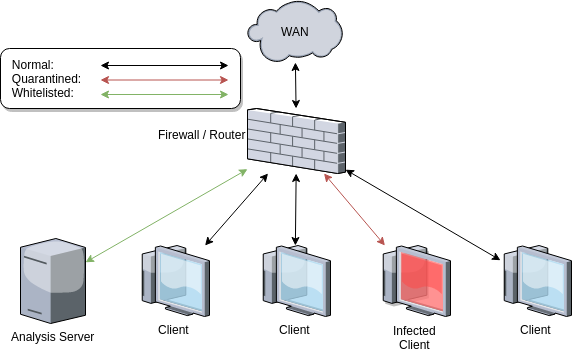
\includegraphics[width=\linewidth]{images/quarantine.png}
			\caption{A simple network example.}
			\label{fig:quarantine}
		\end{figure}
	
		Figure \ref{fig:quarantine} shows a simple network example, where all clients share a single subnet. In this scenario, one client has performed a scan which the analysis server has determined to contain malicious files and has subsequently quarantined the client. The network traffic rules have been displayed in the figure as color coded arrows. 
		
		The 'clean' clients may communicate along the black and green connections allowing them to access the analysis server, the internet and other 'clean' clients though any transmission to the infected client will be dropped by the firewall.
		
		The infected client may only communicate with the router and any client connected via a green connection. Therefore it may not access the internet, or any other non-whitelisted client on the network.\\
		
		\begin{figure}[H]
			\begin{verbatim}
			iptables -F Forward
			iptables -I Forward -d AnalysisServerIP -j ACCEPT
			iptables -I Forward -d WhitelistedServiceIP -j ACCEPT
			iptables -I Forward 3 -s InfectedClientIP -j REJECT
			\end{verbatim}
			\caption{Sample iptables commands generated by the firewall.}
			\label{fig:quarantinerules}
		\end{figure}
	
		As the firewall system loads, it first clears the existing rules to ensure previous entries will not interfere with its operation. Since iptables operates using the first matching rule, the whitelisted ip addresses are then added to ensure all clients may access these services before any clients which were quarantined before the system was shutdown are added with the reject action to prevent the traffic originating from these from being forwarded on to their destination. An example of the commands executed on the system to achieve this operation are displayed in figure \ref{fig:quarantinerules}.
		
	\section{Optimisations to the C4.5 Algorithm}
		Though the C4.5 algorithm described in section \ref{c45} is designed to be fast, a number of optimisations were required to speed up its operation further, and to reduce memory requirements for the generation of large trees.
	
		Firstly, since the implementation of the algorithm used calculates the entropy of a discrete feature by the number of data elements which share the same value, each data element is expected to store a value for each feature. When hundreds of thousands of Boolean features are present this results in an extremely sparse matrix massively increasing the memory requirements to generate the final decision tree. To overcome this issue, the implementation was expanded to allow features to be specified with a Boolean type, which when calculating the entropy will instead determine the value of a feature through its existence in a HashSet of labels in a data element.
	
		Also, due to the scale of the scenarios in which we will be using the algorithm, it was also preferable for the algorithm implementation to support multithreading. To enable the algorithm to utilise multithreading self-contained sections of code were located to be spread across the available threads. Through the use of the Java profiling tool JProfiler, it could be seen that the most frequently executed code was the calculation of entropy of a feature during the process in deciding the most profitable feature to split the data elements. By instead splitting the features into smaller groups, the best feature of each group could be identified, once all groups had completed execution the overall best feature could be found. Through this approach, the training time of one data set was reduced from thirteen hours to just below two, though this increase would also depend on the number of threads available to the computer at the time.
	
		In the C4.5 algorithm, three base cases exist to the creation of a terminal node of the decision tree. One such base case is used to prevent overfitting of the dataset and creates a terminal node with the majority classification of the dataset should the number of data elements be below a specified threshold. From this it can be seen that any feature that occurs in data elements less than this threshold, will not massively influence the final tree as the resulting subsets of data elements will then be transformed into a terminal node due to the satisfaction of the base case.
		

\chapter{Evaluation}
	
	\section{Accuracy}
		As the system will quarantine clients which are seen to be infected with malware, the modules should aim to be as accurate as possible. A false positive could delay the workflow of a user while a false negative could allow malware to go undetected potentially damaging the business infrastructure and its data.
	
		To measure the accuracy of the modules 5000 clean, and 5000 malicious files were scanned by the system. All files used were Portable Executable files sampled at random from the VirusShare \cite{virusshare} database.
		
		\subsection{Import Analysis}
		As can be seen in table \ref{fig:importaccuracy}, the import analysis module has an accuracy of 95.61\%. While this accuracy is relatively high for an experimental technique, in a production environment where thousands of files are scanned routinely, the false positive rate of 5.7\% could cause unnecessary quarantining.
		
		\begin{center}
			\begin{table}
				\begin{tabular}{l|l|c|c|c}
					\multicolumn{2}{c}{}&\multicolumn{2}{c}{Prediction}&\\
					\cline{3-4}
					\multicolumn{2}{c|}{}&Clean&Malware&\multicolumn{1}{c}{Total}\\
					\cline{2-4}
					\multirow{2}{*}{Actual Classification}& Clean & $4715$ & $285$ & $5000$\\
					\cline{2-4}
					& Malware & $154$ & $4846$ & $5000$\\
					\cline{2-4}
					\multicolumn{1}{c}{} & \multicolumn{1}{c}{Total} & \multicolumn{1}{c}{$4869$} & \multicolumn{1}{c}{$5131$} & \multicolumn{1}{c}{}\\
				\end{tabular}
				\caption{Confusion matrix of samples using the Function Import Analysis module.}
				\label{fig:importaccuracy}
			\end{table}		
		\end{center}

	
		\subsection{Yara Rules}
		Table \ref{fig:yaraaccuracy} shows a confusion matrix of the results of scanning the 10000 testing files using the Yara Rules / Byte Matching module. As shown by the results, the module is 98.18\% accurate with only a 0.91\% false negative rate. 
	
		
		\begin{center}
			\begin{table}
				\begin{tabular}{l|l|c|c|c}
					\multicolumn{2}{c}{}&\multicolumn{2}{c}{Prediction}&\\
					\cline{3-4}
					\multicolumn{2}{c|}{}&Clean&Malware&\multicolumn{1}{c}{Total}\\
					\cline{2-4}
					\multirow{2}{*}{Actual Classification}& Clean & $4863$ & $137$ & $5000$\\
					\cline{2-4}
					& Malware & $45$ & $4955$ & $5000$\\
					\cline{2-4}
					\multicolumn{1}{c}{} & \multicolumn{1}{c}{Total} & \multicolumn{1}{c}{$4908$} & \multicolumn{1}{c}{$5092$} & \multicolumn{1}{c}{}\\
				\end{tabular}
				\caption{Confusion matrix of samples using the Yara Rules Analysis module.}
				\label{fig:yaraaccuracy}
			\end{table}
		\end{center}
	
		\subsection{Commercial Product Comparison}
		Since the accuracy is often one of the primary advertised features in a commercial antivirus product, the accuracy of the solution developed was compared against Malwarebytes Anti-Virus and Windows Defender.
		
		

	\section{Speed}
		1000 Malicious Files:
			Combined:
				Time: 668.45 seconds
				Detected: 991
				
	
	\section{Antivirus Comparison}

\chapter{Conclusion}

	\section{Future Improvements}
		\subsection{NetProtect Analysis Server} \label{FutureImprovements.AnalysisServer}
			\subsubsection{Combined Technique Analysis Module}
			The combined module implemented simply carries out the feature extraction procedures of each of the implemented scanning modules in turn. This approach increases the scan time but allows more opportunities to detect the malicious files however suffers from an increased chance of false positives since only one module is required to vote malicious no matter the number who vote for the classification of clean.
			
			A better approach may involve weighting each analysis module based on its accuracy and having each vote on the classification of the file, 0 for clean and 1 for malware. The final classification would then be made through the use of the weighted sum of these votes being above, or below a given threshold. 
			
		\subsection{NetProtect Firewall Server} \label{FutureImprovements.NetworkQuarantine}
			The current implementation of the network quarantine function relies on the quarantining of devices from the network by their assigned ip address. This system is flawed in that an infected client could simply request a new ip address from the DHCP server. This can be remedied with static DHCP binding to ensure clients always receive the same ip address though it would be more beneficial for the firewall server to replace the use of infected host ip addresses in iptables rules with a MAC address filter instead. However, it is not trivial for the server to obtain this information from the connected client, though one method to be considered may be to retrieve the MAC address from the server's ARP table.

\begin{appendices}
	\chapter{Appendix A}
	\section{Sample Counts}
	\begin{table}[H]
		\centering
		\begin{tabular}{lc}
			\toprule
			Format&Count\\
			\midrule
			HTML document&176331\\
			PE32 executable&58070\\
			gzip compressed data&11846\\
			ASCII text&2834\\
			ELF&2793\\
			data&2319\\
			Zip archive data&2291\\
			RAR archive data&553\\
			XML 1.0 document&551\\
			Composite Document File V2 Document&550\\
			Macromedia Flash data (compressed)&538\\
			\bottomrule
			Other&3286\\
			\bottomrule
		\end{tabular}
		\caption{Malicious sample counts for various filetypes.}
		\label{tbl:samplecount}
	\end{table}

	\begin{table}[H]
		\centering
		\begin{tabular}{lc}
			\toprule
			Format&Count\\
			\midrule
			ASCII text&100677\\
			data&47289\\
			XML 1.0 document&43137\\
			PE32 executable&42899\\
			Python script&32809\\
			python 3.6 byte-compiled&27370\\
			PNG image data&27211\\
			PE32+ executable&23053\\
			Ruby script&21015\\
			C source&20037\\
			HTML document&16206\\
			C++ source&9731\\
			UTF-8 Unicode text&8579\\
			Perl5 module source&6566\\
			Java archive data (JAR)&6347\\
			current ar archive&5795\\
			python 2.7 byte-compiled&5549\\
			UTF-8 Unicode (with BOM) text&5087\\
			\bottomrule
			Other&68315\\
			\bottomrule
		\end{tabular}
		\caption{Clean sample counts for various filetypes.}
		\label{tbl:cleancount}
	\end{table}	
	
				
						
	\chapter{Appendix B}
	
	\section{C4.5 Tree - Yara Rules}
	\begin{figure}[H]
		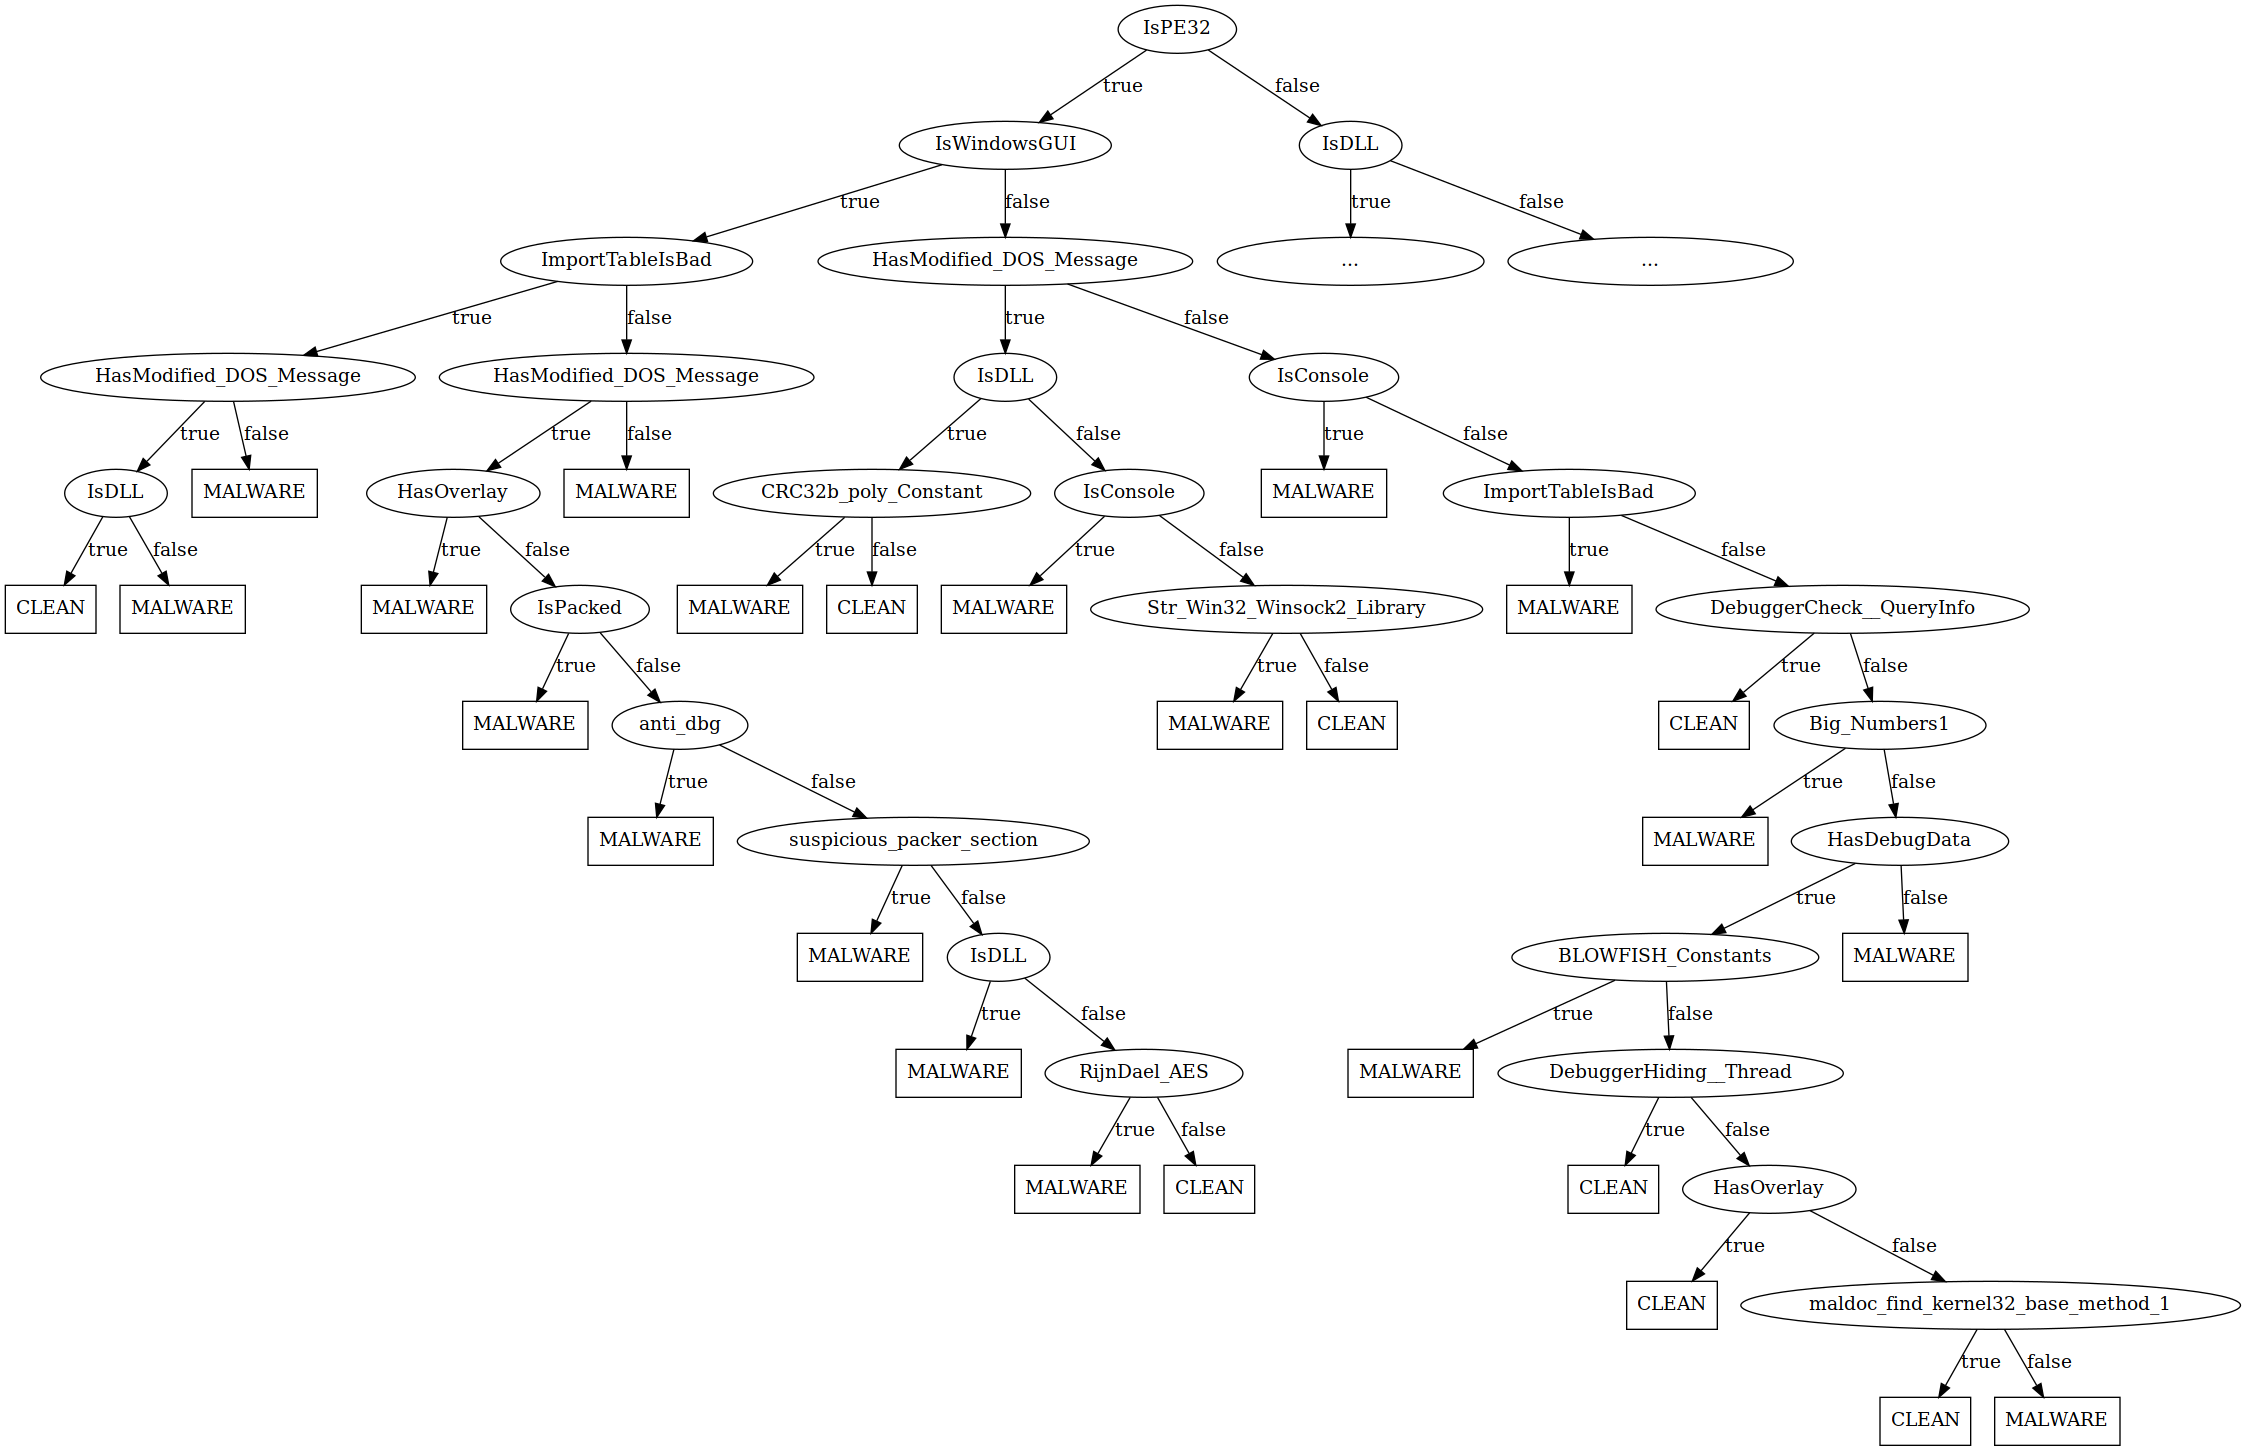
\includegraphics[width=\linewidth]{images/yaratree.png}
				\caption{A subset of the decision tree generated using C4.5 on extracted YARA rules.}
		\label{fig:yaratree}
	\end{figure}

	\section{C4.5 Tree - Function Import Heuristics}
	\begin{figure}[H]
		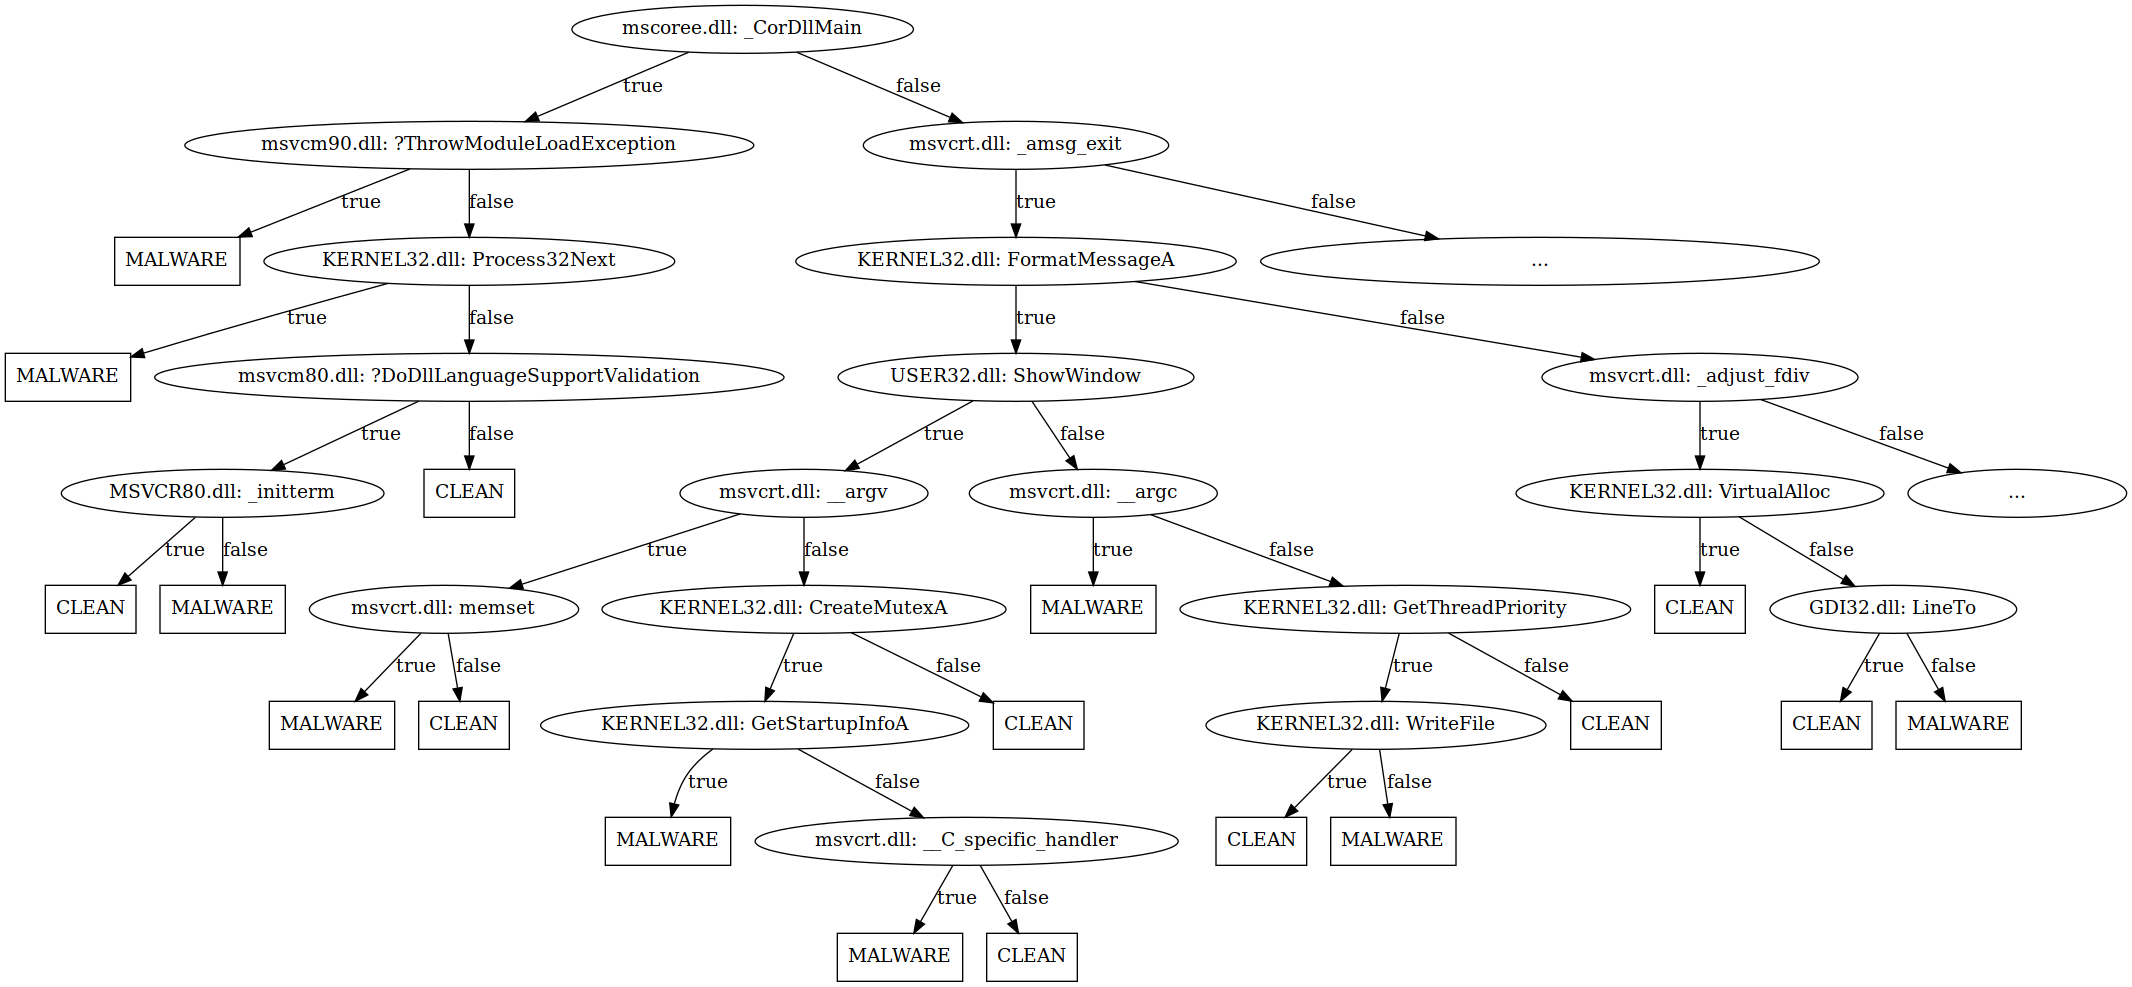
\includegraphics[width=\linewidth]{images/importtree.png}
		\caption{A subset of the decision tree generated using C4.5 on function imports.}
				\label{fig:functionimports}
	\end{figure}
\end{appendices}

\newpage
\printbibliography[title={References}]


\end{document}
